In this chapter we develop a technique for approximating the distribution over failure trajectories. We construct a state-dependent disturbance policy that, when rolled out, causes the system to fail. The distribution over failures allows us to sample a diverse set of likely failures as well as efficiently compute the probability of failure. We start by showing that a sampling distribution that is proportional to the probability of failure is an efficient proposal distribution, and is exactly the distribution over failures when the environment is deterministic. We then describe how to compute the probability of failure using a Bellman equation and approximate it using neural networks and local linear interpolation. Through experiments in the gridworld and T-intersection environments, we show that even when the estimate of the probability of failure has a large amount of error, we still obtain an efficient proposal distribution.

\section{Motivation}

% Why we care about a good failure distribution
In the analysis of safety-critical autonomous systems, the tools of falsification and most-likely failure analysis may not be sufficient to certify the safety of system. They can merely demonstrate that the system is unsafe by finding failure examples. For complex cyber-physical systems, some failures will almost surely exist, and certification will depend on how likely it is for a system to fail. For this reason, we need to develop effective techniques to estimate the probability of failure of an autonomous system, which means creating a distribution over disturbances that causes the most likely failures to occur. 

In addition to the goal of efficient estimation, having a distribution over failures is helpful in the development of safety-critical autonomous systems. If an autonomous system is developed through machine learning, then its ability to navigate dangerous scenarios will likely depend on how many dangerous examples it was trained on. A distribution that produces a diverse set of dangerous scenarios could be used to improve the safety of such systems. 

The difference between the three safety validation tasks is further illustrated in \cref{fig:dof_comparison_safetytasks}. In \cref{fig:dof_policy} we show the expert policy of an agent navigating a simple gridworld with stochastic transitions. When we apply falsification (\cref{fig:dof_falsification}), we find a failure trajectory that is extremely unlikely because falsification algorithms do not consider the probability of the disturbance. We can partially remedy the situation by performing a most-likely failure analysis to arrive at the trajectory shown in \cref{fig:dof_mostlikely_failure}. Although this failure is the one most likely to occur, it cannot be used to estimate the probability that the system fails and only provides a single example that could be used for improving the system performance. Instead, if we can compute the distribution over failures, that is, sample 
\begin{equation}
    \vec{x} \sim p(\vec{x} \mid f(\vec{x}) \not \in \psi) \text{,}
\end{equation}
then we produce many different failure examples, all with relatively high likelihood. \cref{fig:dof_dof} shows samples from the distribution over failures which was computed using techniques developed in the rest of this chapter. 

%What. is wrong with existing approaches
Estimating the distribution over failures is synonymous with finding an efficient proposal distribution for estimating the probability of failure. Importance sampling approaches for estimating the optimal proposal distribution (as discussed in \cref{sec:is}) are limited by the fact that they produce samples of the entire disturbance trajectory $\vec{x}$ and do not have a way of incorporating the environment state. A distribution that does not depend on the environment state will perform poorly in settings where the initial state of the environment or the state transitions are stochastic. To handle these settings, we want to develop a sampling distribution that depends upon the environment state and approximates the distribution over failures.

% Outline our approach
In the rest of the chapter, we propose a stochastic disturbance policy $q(x \mid s)$ that, when applied to a safety validation problem, approximately generates failures from the distribution over failures. If the safety validation problem is deterministic, we find that the optimal disturbance policy is $q^*(x \mid s) \propto p(x \mid s) P_{\rm fail}(s')$ where $P_{\rm fail}(s')$ is the probability that the system fails from the state $s'$ reached by applying disturbance $x$ in state $s$. We use this optimal policy as a motivation for a general policy that can be used in the non-deterministic case. We show that this distribution lowers the variance of an estimator of the probability of failure compared to a basic Monte Carlo approach. 

\begin{figure*}
    \centering
    \begin{subfigure}[b]{0.45\textwidth}
        \centering
        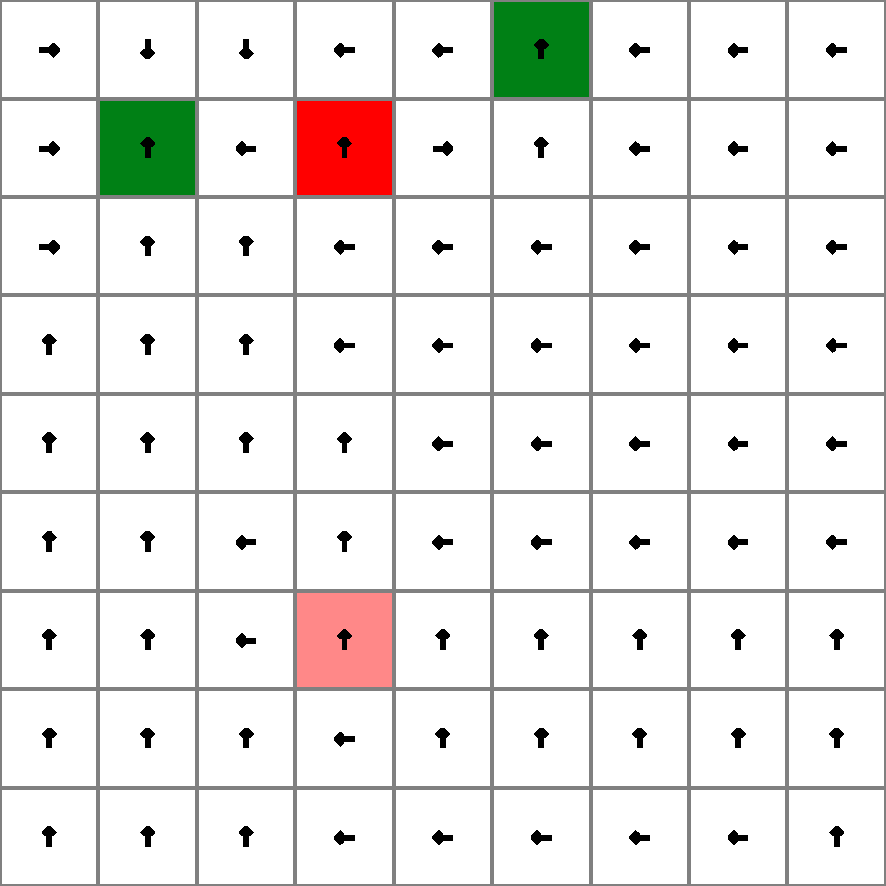
\includegraphics[width=\textwidth]{figures/distribution_over_failures/policy.pdf}
        \caption{Expert policy.}
        \label{fig:dof_policy}
    \end{subfigure}
    \hfill
    \begin{subfigure}[b]{0.45\textwidth}
        \centering
        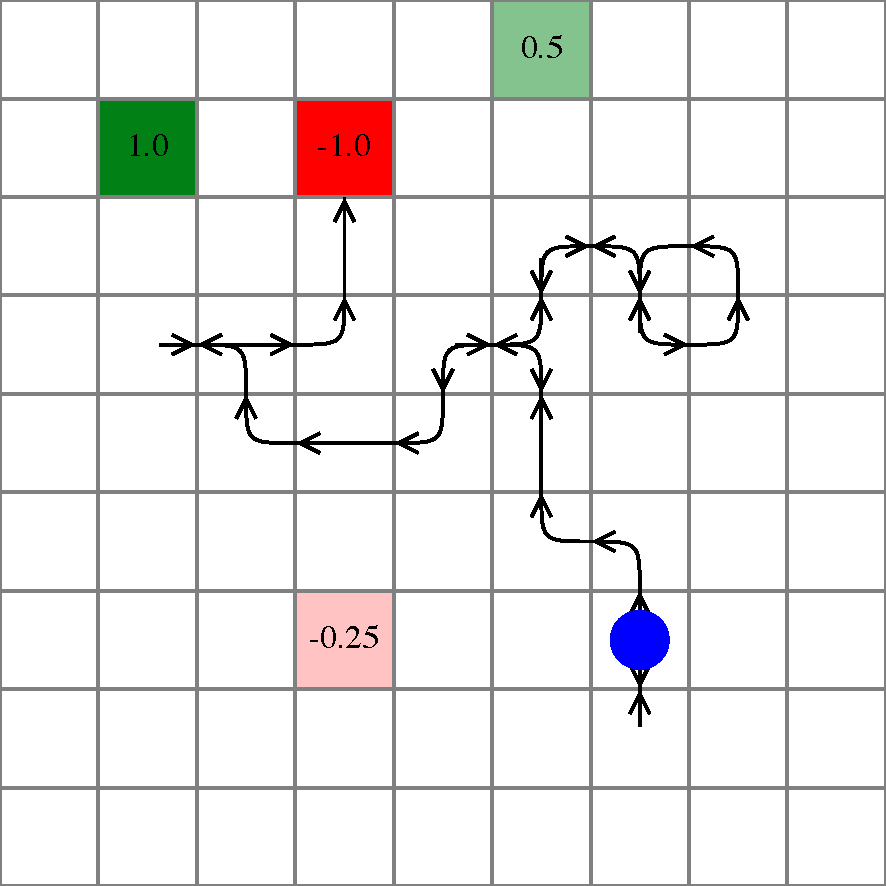
\includegraphics[width=\textwidth]{figures/distribution_over_failures/falsification_failure.pdf}
        \caption{Failure from falsification.}
        \label{fig:dof_falsification}
    \end{subfigure}
    \begin{subfigure}[b]{0.45\textwidth}
        \centering
        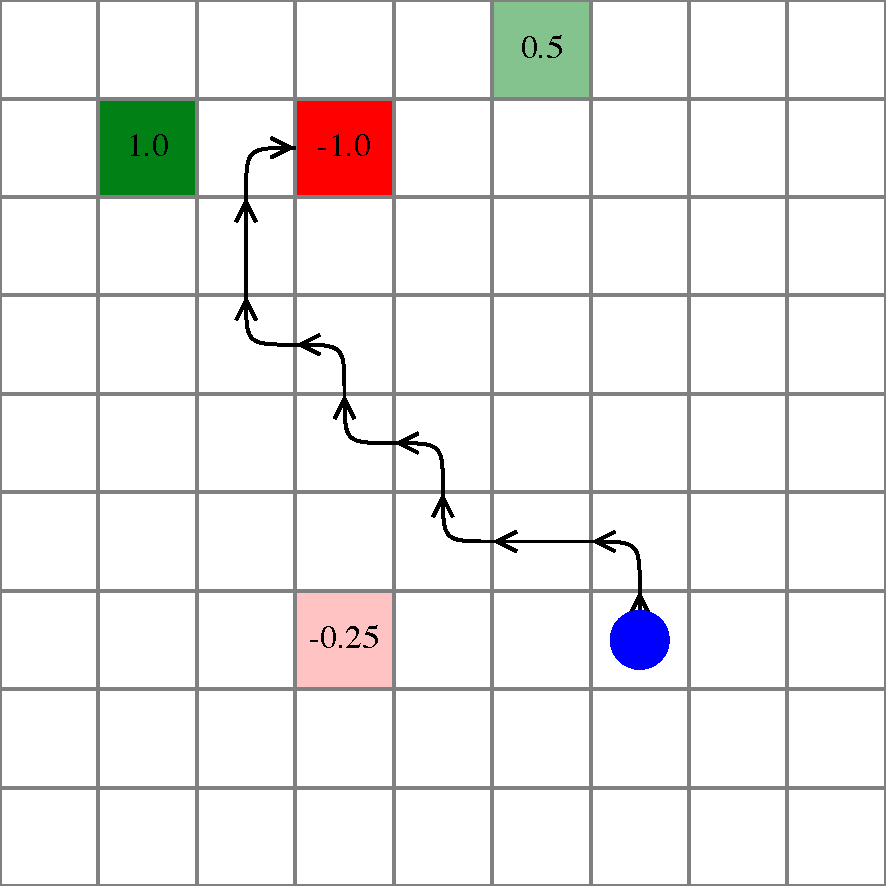
\includegraphics[width=\textwidth]{figures/distribution_over_failures/most_likely_failure.pdf}
        \caption{Most-likely failure.}
        \label{fig:dof_mostlikely_failure}
    \end{subfigure}
    \hfill
    \begin{subfigure}[b]{0.45\textwidth}
        \centering
        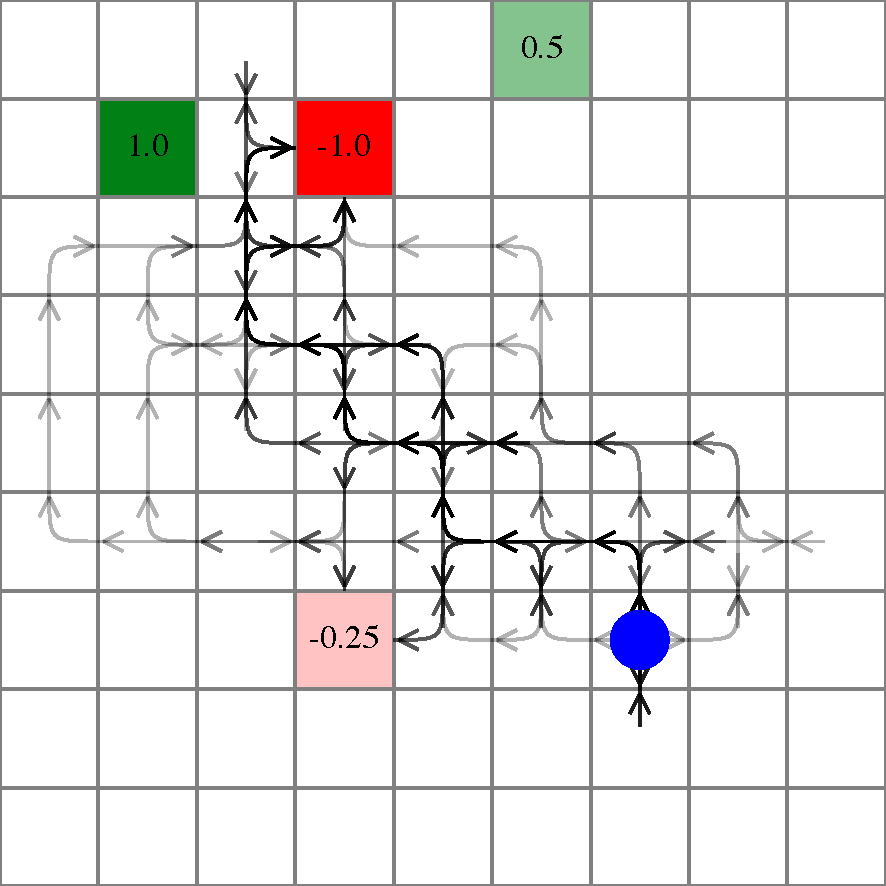
\includegraphics[width=\textwidth]{figures/distribution_over_failures/distribution_over_failures.pdf}
        \caption{Samples from failure distribution.}
        \label{fig:dof_dof}
    \end{subfigure}
    \caption{Comparison of safety validation tasks.}
    \label{fig:dof_comparison_safetytasks}
\end{figure*}


\section{State-Dependent Importance Sampling}
This section describes the problem of constructing a state-dependent importance sampling distribution for efficiently estimating the probability of failure of a system. We first describe the sampling problem and then  propose a state-dependent disturbance distribution that produces low-variance estimates of the probability of failure. Through an analysis of variance, we show that our proposed distribution is optimal when the system and environment are deterministic given the disturbances.

\subsection{Problem Setup}
% Definition of notation
Suppose we wish to estimate the probability of failure $P_{\rm fail}$ of a system in an environment with states $s \in S$, subject to disturbances $x \in X$. A trajectory is $\vec{\tau} = [s_0, x_1, s_1, \ldots x_{t_{\rm max}}, s_{t_{\rm max}}]$ and has probability $p(\vec{\tau})$, which models the likelihood of state transitions and disturbances. A trajectory is a failure if the sequence of states violates the safety specification $\psi$ and we denote a failure trajectory of both states and disturbances as $\vec{\tau} \not \in \psi$. 

% rehashing of importance sampling theory
For importance sampling, we wish to develop a proposal distribution $q(\vec{\tau})$ that estimates the probability of failure with the minimal number of samples. An unbiased estimator of the probability of failure can be computed from $N$ independent samples $\vec{\tau}_i \sim q(\vec{\tau})$ as
\begin{equation}
\hat{P}_{\rm fail} = \frac{1}{N} \sum_{i=1}^N \frac{p(\vec{\tau}_i) \mathds{1}{\{ \vec{\tau}_i \not \in \psi \}}}{q(\vec{\tau}_i)} \text{,} \label{eq:pfail_estimator}
\end{equation}
where $\mathds{1}$ is the indicator functions. 

The variance of $\hat{P}_{\rm fail}$ is given by
\begin{align}
\text{Var}_q\left[ \hat{P}_{\rm fail} \right] &= \frac{1}{N} \left( \mathbb{E}_q \left[\left(\frac{p(\vec{\tau}) \mathds{1}{\{ \vec{\tau} \not \in \psi \}}}{q(\vec{\tau})} \right)^2 \right] - \mathbb{E}_q\left[ \frac{p(\vec{\tau}) \mathds{1}{\{ \vec{\tau} \not \in \psi \}}}{q(\vec{\tau})}  \right]^2 \right) \label{eq:var_estimator}\\
&= \frac{1}{N} \left(\mathbb{E}_p \left[\frac{p(\vec{\tau}) \mathds{1}{\{ \vec{\tau} \not \in \psi \}}}{q(\vec{\tau})} \right] - P_{\rm fail}^2 \right)\label{eq:pfail_variance}
\end{align}
where have used the fact that the estimator is unbiased so $\mathbb{E}_q\left[ \hat{P}_{\rm fail}  \right] = P_{\rm fail}$. From importance sampling theory (and by inspection of \cref{eq:var_estimator}), we know that the minimum variance proposal distribution is given by 
\begin{equation}
    q^*(\vec{\tau}) = \frac{p(\vec{\tau}) \mathds{1}{\{ \vec{\tau} \not \in \psi \}}}{P_{\rm fail}} \text{.}
\end{equation}

% Form of the proposal distribution
In safety validation of sequential decision-making problems, we cannot directly sample trajectories $\vec{\tau}$ of the system. Instead, the adversary influences the trajectories through the choice of disturbance. We must therefore define a distribution over disturbances that depends only on the trajectory at earlier timesteps and not future ones. We construct a distribution over the disturbance at time $t$ with the form
\begin{equation}
    q(x_t, \mid \vec{\tau}_{0:t-1})
\end{equation}
where $\vec{\tau}_{0:t} = [s_0, x_1, s_1, \ldots, x_t, s_t]$. The full distribution over trajectories is constructed as
\begin{equation}
    q(\vec{\tau}) = p(s_0) \prod_{t = 1}^{t_{\rm max}} p(s_t \mid \vec{\tau}_{0:t-1}, x_t) q(x_t, \mid \vec{\tau}_{0:t-1}) \text{.} \label{eq:induced_distribution}
\end{equation}

\subsection{Proposal distribution}

% Defining the proposal distribution
We now present a proposal distribution that reduces the variance of $\hat{P}_{\rm fail}$ compared to Monte Carlo sampling and is optimal in the deterministic setting. Define the disturbance policy
\begin{equation}
    q^*(x_t, \mid \vec{\tau}_{0:t-1}) = \frac{p(x_t \mid \vec{\tau}_{0:t-1}) P_{\rm fail}(\vec{\tau}_{0:t-1}, x_t)}{P_{\rm fail}(\vec{\tau}_{0:t-1})} \text{,} \label{eq:disturbance_policy}
\end{equation}
where $P_{\rm fail}(\vec{\tau}_{0:t})$ is the probability that the system fails under the distribution $p(\vec{\tau})$ given the sequence $\vec{\tau}_{0:t}$. The full proposal distribution over trajectories is given by 
\begin{align}
    q^*(\vec{\tau}) &= p(s_0) \prod_{t=1}^{t_{\rm max}} \frac{p(s_t \mid \vec{\tau}_{0:t-1}, x_t)  p(x_t \mid \vec{\tau}_{0:t-1}) P_{\rm fail}(\vec{\tau}_{0:t-1}, x_t)}{P_{\rm fail}(\vec{\tau}_{0:t-1})} \\
    &= p(\vec{\tau}) \prod_{t=1}^{t_{\rm max}} \frac{P_{\rm fail}(\vec{\tau}_{0:t-1}, x_t)}{P_{\rm fail}(\vec{\tau}_{0:t-1})} \text{.} \label{eq:full_proposal}
\end{align}

At first, it may seem circular to define a proposal distribution that depends upon the very quantity we are trying to estimate (the probability of failure). Our goal is not just to estimate the probability of failure, but to construct a distribution that we can sample failures from.  Additionally, we will show through experimentation that an efficient proposal distribution can be constructed with even a rough estimate of the probability of failure at each state. For the following analysis we assume we know the probability of failure exactly and that the states and disturbances are discrete. A similar analysis may be performed for continuous variables by appropriately converting sums to integrals.

\begin{proposition} 
The disturbance policy $q^*(x_t, \mid \vec{\tau}_{0:t-1})$ induces a valid probability distribution over trajectories.
\end{proposition}

\begin{proof}
To show this, we need to show that $q^*(x_t, \mid \vec{\tau}_{0:t-1})$ is a valid probability distribution and $q^*(\vec{\tau})$ will be valid by construction from \cref{eq:induced_distribution}. First we note that $P_{\rm fail}(\cdot) \in [0,1]$ and $p(x_t \mid \vec{\tau}_{0:t-1}) > 0$ so $q^*(x_t, \mid \vec{\tau}_{0:t-1})$ is non-negative for all disturbances $x_t$. Then we can show proper normalization by using a recursive definition of the probability of failure, given by 
\begin{equation}
    P_{\rm fail}(\vec{\tau}_{0:t-1}) = \sum_{x_t} p(x_t \mid \vec{\tau}_{0:t-1}) P_{\rm fail}(\vec{\tau}_{0:t-1}, x_t) \text{.}
\end{equation}
Thus
\begin{align}
    \sum_{x_t} q^*(x_t, \mid \vec{\tau}_{0:t-1}) &= \sum_{x_t} \frac{p(x_t \mid \vec{\tau}_{0:t-1}) P_{\rm fail}(\vec{\tau}_{0:t-1}, x_t)}{P_{\rm fail}(\vec{\tau}_{0:t-1})} \\
    &= \frac{P_{\rm fail}(\vec{\tau}_{0:t-1})}{P_{\rm fail}(\vec{\tau}_{0:t-1})} \\
    &= 1
\end{align}
\end{proof}

If we use the disturbance policy to sample trajectories $\vec{\tau}$ and use them to estimate the probability of failure, we need to understand the variance of the estimate. A good proposal distribution will produce estimates that have lower variance than estimates computed from the true distribution $p(\vec{\tau})$.

\begin{proposition}
The variance of the failure probability estimate (\cref{eq:pfail_estimator}) under the proposal distribution $q^*$ is
\begin{align}
    \text{Var}_{q^*}\left[ \hat{P}_{\rm fail} \right] &= \frac{P_{\rm fail}^2}{N} \left( \mathbb{E}_{p_{\tau \mid \mathds{1} \{\vec{\tau} \not \in \psi\}}}  \left[ \prod_{t=0}^{t_{\rm max}} \frac{p(s_t \mid \vec{\tau}_{0:t-1}, x_t, \mathds{1} \left\{ \vec{\tau} \not \in \psi \right\})}{p(s_t \mid \vec{\tau}_{0:t-1}, x_t)} \right] - 1 \right) \text{,}
    % \\
    % &= \frac{P_{\rm fail}^2}{N} \left( \mathbb{E}_{p_{\tau \mid \mathds{1} \{\vec{\tau} \not \in \psi\}}}  \left[ \prod_{t=1}^{t_{\rm max}} \frac{P_{\rm fail}(\vec{\tau}_{0:t})}{P_{\rm fail}(\vec{\tau}_{0:t-1}, x_t)} \right] - 1 \right) \\
\end{align}
\end{proposition}

\begin{proof}
To show this, we can start by substituting \cref{eq:full_proposal} into \cref{eq:pfail_variance} to get
\begin{equation}
    \text{Var}_{q^*}\left[ \hat{P}_{\rm fail} \right] = \frac{1}{N} \left(\mathbb{E}_p \left[\mathds{1}\{ \vec{\tau} \not \in \psi \} \prod_{t=1}^{t_{\rm max}} \frac{P_{\rm fail}(\vec{\tau}_{0:t-1})}{P_{\rm fail}(\vec{\tau}_{0:t-1}, x_t)} \right] - P_{\rm fail}^2 \right) \label{eq:starting_variance_expression}
\end{equation}
Then, applying Bayes' rule we have 
\begin{equation}
    P_{\rm fail}(\vec{\tau}_{0:t}) = \frac{p(\vec{\tau}_{0:t} \mid \mathds{1} \left\{ \vec{\tau} \not \in \psi \right\}) P_{\rm fail}}{p(\vec{\tau}_{0:t})} \text{.}
\end{equation}
When substituted into the ratio term in \cref{eq:starting_variance_expression} we get
\begin{align}
    \prod_{t=1}^{t_{\rm max}} \frac{P_{\rm fail}(\vec{\tau}_{0:t-1})}{P_{\rm fail}(\vec{\tau}_{0:t-1}, x_t)} &= \prod_{t=1}^{t_{\rm max}} \frac{p(\vec{\tau}_{0:t-1} \mid \mathds{1} \left\{ \vec{\tau} \not \in \psi \right\}) p(\vec{\tau}_{0:t-1}, x_t)}{p(\vec{\tau}_{0:t-1}, x_t \mid \mathds{1} \left\{ \vec{\tau} \not \in \psi \right\}) p(\vec{\tau}_{0:t-1})} \\
    &= \prod_{t=1}^{t_{\rm max}} \frac{p(x_t \mid \vec{\tau}_{0:t-1})}{p(x_t \mid \vec{\tau}_{0:t-1}, \mathds{1} \left\{ \vec{\tau} \not \in \psi \right\})} \\
    &= \prod_{t=1}^{t_{\rm max}} \frac{p(x_t, s_t \mid \vec{\tau}_{0:t-1})p(s_t \mid \vec{\tau}_{0:t-1}, x_t, \mathds{1} \left\{ \vec{\tau} \not \in \psi \right\})}{p(x_t, s_t \mid \vec{\tau}_{0:t-1}, \mathds{1} \left\{ \vec{\tau} \not \in \psi \right\})p(s_t \mid \vec{\tau}_{0:t-1}, x_t)} \\
    &= \frac{p(\vec{\tau})}{p(\vec{\tau} \mid \mathds{1} \left\{ \vec{\tau} \not \in \psi \right\})} \prod_{t=0}^{t_{\rm max}} \frac{p(s_t \mid \vec{\tau}_{0:t-1}, x_t, \mathds{1} \left\{ \vec{\tau} \not \in \psi \right\})}{p(s_t \mid \vec{\tau}_{0:t-1}, x_t)} \\
    &= P_{\rm fail}\prod_{t=0}^{t_{\rm max}} \frac{p(s_t \mid \vec{\tau}_{0:t-1}, x_t, \mathds{1} \left\{ \vec{\tau} \not \in \psi \right\})}{p(s_t \mid \vec{\tau}_{0:t-1}, x_t)} \label{eq:simplified_ratio}
\end{align}
where we have used the fact $p(\vec{\tau} \mid \mathds{1} \left\{ \vec{\tau} \not \in \psi \right\}) =  p (\vec{\tau})/P_{\rm fail}$ to get \cref{eq:simplified_ratio}. Finally, we get the desired result by plugging \cref{eq:simplified_ratio} into \cref{eq:starting_variance_expression} and applying the identity
\begin{align}
    \mathbb{E}_p \left[ \mathds{1} \{\vec{\tau} \not \in \psi\} f(\vec{\tau}) \right] &= \mathbb{E}_p \left[ \mathds{1} \{\vec{\tau} \not \in \psi\} \right] \mathbb{E}_{p_{\vec{\tau} \mid \mathds{1} \{\vec{\tau} \not \in \psi\}}}  \left[ f(\vec{\tau}) \right]  \\
    &= P_{\rm fail} \mathbb{E}_{p_{\vec{\tau} \mid \mathds{1} \{\vec{\tau} \not \in \psi\}}}  \left[ f(\vec{\tau}) \right]\text{.}
\end{align}
\end{proof}

The variance of the estimator from $q^*$ differs from the Monte Carlo estimator by the term
\begin{equation}
    \mathbb{E}_{p_{\tau \mid \mathds{1} \{\vec{\tau} \not \in \psi\}}}  \left[ \prod_{t=1}^{t_{\rm max}} \frac{p(s_t \mid \vec{\tau}_{0:t-1}, x_t, \mathds{1} \left\{ \vec{\tau} \not \in \psi \right\})}{p(s_t \mid \vec{\tau}_{0:t-1}, x_t)} \right] \text{.}
\end{equation}
We note that this term is always greater than $1$ and is maximized when the choice of disturbance has no influence on the next state of the environment. In that case, $P_{\rm fail}(\vec{\tau}_{0:t-1}) = P_{\rm fail}(\vec{\tau}_{0:t-1}, x_t)$ and we can see from  \cref{eq:starting_variance_expression}, that the variance increases to the Monte Carlo estimate. The less stochasitic the environment is given the state, the smaller the variance of the estimator. In the case where each state transition is deterministic given the disturbance, we have $p(s_t \mid \vec{\tau}_{0:t-1}, x_t, \mathds{1} \left\{ \vec{\tau} \not \in \psi \right\}) = p(s_t \mid \vec{\tau}_{0:t-1}, x_t)$, and the variance goes to zero, indicating that $q^*$ is the optimal importance sampling distribution. 

Assuming the environment does not have too much uncontrolled stochasticity, we can approximate the distribution over failures by sampling disturbances according to $q^*$. To compute $q^*$ we need $p(x \mid s)$, which is given, and $P_{\rm fail}(\cdot)$.  The following section describes how to efficiently compute the probability of failure as a function of the state when we can make the Markov assumption.


\section{Estimating the Probability of Failure}

An efficient proposal distribution can computed using an estimate of the probability of failure for each trajectory segment. Estimating the probability of failure over the distribution of trajectories could quickly become intractable due to the dimensionality of the space of trajectories. The computation can be significantly simplified if we assume that the system and environment are Markov so the probability of failure only depends on the current state and the choice of the next diturbance. The Markov version of all the equations in the previous section can be obtained by letting $\vec{\tau}_{0,t} = s_t$ .

With the Markov assumption, the probability of failure satisfies the Bellman equation
\begin{equation}
    P_{\rm fail}(s) = \begin{cases}
    1 & s \in S_{\rm fail} \\
    0 & s \in S_{\rm term} \text{ and } s \not \in S_{\rm fail} \\
    \sum_x p(x \mid s) P_{\rm fail}(s, x) & \text{otherwise}
    \end{cases} \label{eq:ch5_bellman}
\end{equation}
where $S_{\rm fail}$ is the set of failure states, $S_{\rm term}$ is the set of terminal states, and
\begin{equation}
    P_{\rm fail}(s, x) = \sum_{s'} p(s' \mid s, x) P_{\rm fail}(s') \text{.}
\end{equation}
\cref{eq:ch5_bellman} is similar in structure to the Bellman equations that show up in the theory of sequential decision making (i.e. \cref{eq:ch2_bellman_v,eq:ch2_bellman_q}). As such, we can apply many of the same techniques used in reinforcement learning to compute the probability of failure. We now introduce exact and approximate value iteration and Q-learning with neural network function approximation. 

\subsection{Value Iteration}

When the state space of the environment is discrete or easily discretized, we can use exact or approximate value iteration~\cite{dmubook} to compute the probability of failure. Value iteration is a dynamic programming technique that iteratively solves a Bellman equation over a set of states. In exact value iteration, $P_{\rm fail}(s)$ is represented by a table with entries at every state. Exact value iteration is only feasible when the state space is discrete and relatively small. For larger state spaces, approximate value iteration represents $P_{\rm fail}(s)$ by a function. In local approximation value iteration the function is usually constructed from piecewise continuous polynomials that can exactly satisfy the estimated value at a set of sampled states. In global approximation value iteration there is a single function that maps states to values (such as a neural network), so we cannot generally specify the value of given state. 


A general value iteration procedure is outlined in \cref{alg:value_iteration}. It takes as input the set of states $\vec{s}$ (either the complete state space or a finite number of sample states), the set of failure states $S_{\rm fail}$ and the set of terminal states $S_{\rm terminal}$. The algorithm starts by initializing the estimate of the probability of failure at each state (line \ref{line:vi_initialize}), and then iterates until convergence. For each state, we apply the Bellman update operator to compute the target value $y$ (lines \ref{line:vi_start_bellman_update} to \ref{line:vi_summation}). When computing the term on line \ref{line:vi_summation}, we usually estimate $P_{\rm fail}(s, x)$ by sampling a set of next states $s^\prime$ and using an average of the approximation $P_{\rm fail}(s^\prime)$. Lastly, we update the estimate of the probability of failure using the target value. In exact and local approximation value iteration the update simply assigns the value $y$ to the corresponding state. In global approximation value iteration, we typically minimize $L(P(s), y)$ for some loss function $L$. Once the algorithm converges the estimate of the probability of failure is returned (line \ref{line:vi_return}). 

\begin{algorithm}
\caption{Value Iteration for computing the probability of failure.} \label{alg:value_iteration}
\begin{algorithmic}[1]
    \Function{ValueIteration}{$S$, $S_{\rm fail}$, $S_{\rm terminal}$}
        \State $\textproc{Initialize}(P_{\rm fail}(s))$ \label{line:vi_initialize}
        \Loop
            \For{each state $s \in \vec{s}$}
                \If{$s \in S_{\rm fail}$} \label{line:vi_start_bellman_update}
                    \State $y \gets 1$
                \ElsIf{$s \in S_{\rm terminal}$ and $s \not \in S_{\rm fail}$}
                    \State $y \gets 0$
                \Else
                    \State $y \gets \sum_x p(x \mid s) P_{\rm fail}(s,x)$ \label{line:vi_summation}
                \EndIf
                \State \textproc{update}($P_{\rm fail}(s)$, $y$) \label{line:vi_update}
            \EndFor
        \EndLoop
        \State \textbf{return} $P_{\rm fail}(s)$ \label{line:vi_return}
    \EndFunction
\end{algorithmic}
\end{algorithm}

Exact value iteration is guaranteed to converge to the true value function which makes it an appealing algorithm to use, but it has limits in scalability and the types of environments it can work with. Explicitly looping over the set of state excludes environments with large or continuous state spaces. Even a coarse discretization becomes intractable because the number of grid points scales exponentially with the number of state dimensions. Additionally, value iteration requires the ability to initialize a system and environment into a particular state. This requirement may not be feasible more many real-world simulators and it precludes the analysis of non-Markovian systems. We now introduce deep Q-Learning for failure probability estimation, which relaxes these assumptions.


\subsection{Deep Q-Learning}

The DQN algorithm~\cite{mnih2015human} can easily be adapted to compute the probability of failure. The Q-network takes as input the state and outputs the probability of a failure for each disturbance, estimating $P_{\rm fail}(s, x)$. As in value iteration techniques, we start be assigning failure states a value of \num{1} and non-failure terminal states a value of \num{0} We use the same algorithm as \cref{alg:dqn} but alter the target (\cref{eq:ch2_dqn_target}) to be 
\begin{equation}
    y(s, x, s^\prime; \theta^-) = \begin{cases}
    1 & \text{if } s^\prime \in S_{\rm fail} \\ 
    0 & \text{if } s^\prime \not \in S_{\rm fail} \text{ and } s^\prime \in S_{\rm terminal} \\ 
    \sum_{x^\prime}p(x^\prime \mid s) P_{\rm fail}(s^\prime, x^\prime) & \text{otherwise} \\
    \end{cases} \text{.}
\end{equation}
Similar to traditional DQN, we collect new experience samples with an $\epsilon$-greedy approach. We sample a disturbance according to our current estimate of $q^*$ with probability $1-\epsilon$, and with probability $\epsilon$, we sample a random disturbance uniformly at random.

% Using the sigmoid activation
In addition to changing the target and rollout policy, there are a few other changes that are necessary for training a good predictor of the probability of failure. First, we need to ensure that the network output is always between \num{0} and \num{1} to be a valid probability value. The easiest way to force this constraint is to have the last layer of the network be a sigmoid activation given by 
\begin{equation}
    \sigma(z) = \frac{1}{1 + e^{-z}} \text{,}
\end{equation}
which maps the real numbers to the range $(0,1)$. 

% Using the MSLE
When estimating the probability of failure, we must also be careful in our choice of loss function. DQN usually employs the huber loss or the mean squared error loss but these loss functions do not handle differences in small values very well. Even if the network has many orders of magnitude error in a prediction of the probability of failure, the mean squared error of that prediction may still be small. We therefore employ the mean squared log error (MSLE) given by
\begin{equation}
    L_{\rm MSLE}(y, \hat{y}) = \frac{1}{N}\sum_{i=1}^N (\log(y + \epsilon) - \log(\hat{y} + \epsilon))^2
\end{equation}
where $\hat{y}$ is the prediction of $y$ and $\epsilon$ is a small value added for numerical stability. Informally, the MSLE penalizes the relative error instead of the absolute error. 

In traditional DQN with prioritized experience replay, the experience samples are prioritized according to their temporal difference error $|y - \hat{y}|$. Again, this value can be small even when the relative error is large. We therefore make the priority of each sample equal to the difference in the log values $|\log(y + \epsilon) - \log(\hat{y + \epsilon})|$. This alteration allows the network to focus on samples that have large relative error. 

DQN has no explicit dependence on the size of the state space because it gathers data by sampling episodes from a simulator. It can therefore scale to problems with large state spaces and never requires the simulator to be initialized into a particular state, making it more easily applied to large and inflexible simulators or non-Markovian systems. Some drawbacks to DQN are the lack of formal convergence guarantees and the requirement of a discrete disturbance space.

\section{Experiments}
\label{sec:ch5_expr}
This section demonstrates our technique for approximating the distribution over failures of a Markovian system using the state-dependent proposal distribution
\begin{equation}
    q^*(x_t, \mid s_{t-1}) = \frac{p(x_t \mid s_{t-1}) P_{\rm fail}(s_{t-1}, x_t)}{P_{\rm fail}(s_{t-1})} \text{.} \label{eq:markov_disturbance_policy}
\end{equation}
When the ground truth is unavailable, we use the following metrics to evaluate the performance of our proposal distribution:
\begin{itemize}
    \item \emph{Failure rate}: The fraction of failures found when using the proposal distribution
    \begin{equation}
        \frac{1}{N} \sum_{i=1}^N \mathds{1}\left\{ \vec{\tau}_i \not \in \psi \right\}, \quad \vec{\tau}_i \sim q^*(\vec{\tau})
    \end{equation}
    The true distribution over failures would always produce failures, but due to stochasticity in initial conditions and errors in the estimate of the probability of failure, the failure rate is usually less than \num{1}. We want a proposal distribution that returns as many failures as possible. In our experiments, failure rate is estimated with \num{1000} samples. 
    \item \emph{Failure trajectory log-likelihood}: The average log-likelihood of failure trajectories produced with the proposal distribution: 
    \begin{equation}
        \frac{1}{N} \sum_{i=1}^N \log p(\vec{\tau}_i), \quad \vec{\tau}_i \sim q^*(\vec{\tau} \mid \vec{\tau} \not \in \psi) \text{.}
    \end{equation}
    For most-likely failure analysis and estimating the probability of failure, we want a distribution that produces high likelihood failures. In our experiments the log-likelihood of failures is estimated from \num{100} failure trajectories.
    \item \emph{Probability of failure estimate}: The best indicator of an efficient proposal distribution is the ability to estimate the probability of failure with minimal samples. We report the estimate of the probability of failure against the number of samples and \num{99}\% confidence bounds. The confidence bounds are computed from a Beta distribution with the same mean and variance as the estimate.
\end{itemize}

We compare our proposal distribution to three baselines:
\begin{itemize}
    \item \emph{Monte Carlo sampling}: Disturbance trajectories are sampled from the true distribution $p(x \mid s)$.
    \item \emph{Uniform sampling}: Disturbance trajectories are sampled from a uniform distribution over disturbances. 
    \item \emph{Cross entropy method}: We apply the cross entropy method to learn the optimal distribution over disturbances without reference to the state. The distribution was estimated over \num{100} iterations, each with \num{1000} samples and a minimum of \num{100} elite samples.
\end{itemize}

The first set of experiments use the simple gridworld scenario. We first show that the even under a significant amount of error in the estimate of the probability a failure, \cref{eq:markov_disturbance_policy} performs well. We then shown that DQN can effectively model the probability of failure even when the probability of failure is very small. The second set of experiments uses the T-intersection scenario with a single adversary. We show that both local approximation value iteration and DQN outperform baseline methods. 

\subsection{Simple Gridworld}

The first set of experiments involves the simple gridworld scenario because it can be solved using exact value iteration. Access to the ground truth allows us to investigate the effect of errors in the estimate of the probability of failure and the use of approximate algorithms such as DQN. Using the reward distribution shown in \cref{fig:simple_gridworld}, we train an agent to expertly navigate the gridworld subject to a successful transition probability of $p_{\rm success} = 0.999$. We then construct an adversarial gridworld that controls the transitions of the agent and use it for the following experiments.

% Noisy estimates
To investigate the effect of errors in the estimate of the probability of failure we perturb the ground truth $P_{\rm fail}(s)$ and observe its effect on our performance metrics. To compute the noisy probability of failure estimate $\tilde{P}_{\rm fail}(s)$ at state $s$ we independently sample $\delta \mathcal{U}(-\delta_{\rm max}, \delta_{\rm max})$, and then multiply
\begin{equation}
    \tilde{P}_{\rm fail}(s) = 10^\delta P_{\rm fail}(s) \text{.}
\end{equation}
The parameter $\delta_{\rm max}$ specifies the maximum magnitude of error in the estimate of the probability of failure. When $P_{\rm fail}(s)$ is exactly \num{0}, we first initialize it to the smallest nonzero entry in the table and then apply the noise. 

% results
The results of experiments with $\delta_{\rm max} \in [1,2,3]$ are shown in \cref{tab:ch5_gridworld_noise_results} and the estimates of the probability of failure are plotted in \cref{fig:gridworld_pfail_W_noise_vs_samples}. The failure rate of all noisy proposal distributions stays at \num{1} but the log-likelihood begins to degrade significantly with $\delta_{\rm max} = 3$. The estimate of the probability of failure is accurate and relatively low-variance for $\delta_{\rm max} = 1$ and $\delta_{\rm max} = 2$. For  $\delta_{\rm max} = 3$, the estimate is ultimately low, likely due to the prevalence of low log-likelihood failure trajectories. Although only a toy example, these experiments show that a proposal distribution based on $P_{\rm fail}(s)$ may be rather robust to estimation errors. 

\begin{table}
    \centering
    \caption{Performance with noisy estimates of the probability of failure.}
    \label{tab:ch5_gridworld_noise_results}
    \begin{tabular}{@{}lll@{}} 
        \toprule
        \textbf{Noise Level} & \textbf{Failure Rate} & \textbf{Log-Likelihood}\\
        \midrule
        No Noise & \num{1.0} \pm \num{0.0} & \num{-10.894} \pm \num{0.49} \\
        $\delta_{\rm max} = 1$ & \num{1.0} \pm \num{0.0} & \num{-10.493} \pm \num{0.421} \\
        $\delta_{\rm max} = 2$ & \num{1.0} \pm \num{0.0} & \num{-12.254} \pm \num{0.551} \\
        $\delta_{\rm max} = 3$ & \num{1.0} \pm \num{0.0} & \num{-181.049} \pm \num{22.592} \\
        \bottomrule
    \end{tabular}
\end{table}

\begin{figure}
        \centering
        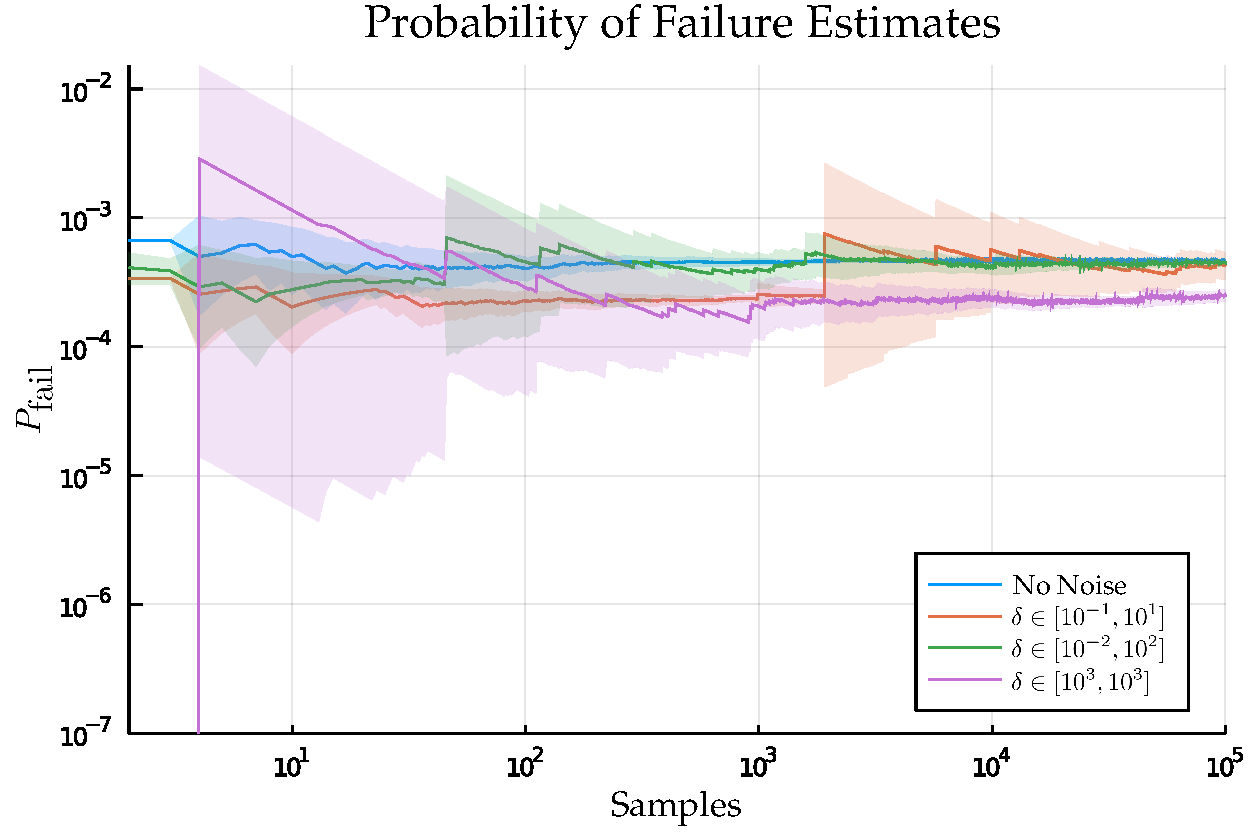
\includegraphics[width=\textwidth]{figures/distribution_over_failures/pfail_gridworld_w_noise.pdf}
        \caption{$P_{\rm fail}$ estimation with varying degrees of noise.}
        \label{fig:gridworld_pfail_W_noise_vs_samples}
\end{figure}


% Use of DQN
Despite the robustness to errors in the estimation of the probability of failure, it is beneficial to construct the best estimate possible. We now investigate the use of DQN as an approximate technique for estimating the probability of failure and compare it to the ground truth. 

We train a neural network that has two hidden layers (\num{64} and \num{32} hidden units and relu activations) and a sigmoid activation for each output node. The network was trained over \num{5e5} iterations with the ADAM optimizer and a learning rate of \num{1e-3}. The neural network represents the function $P_{\rm fail}(s,x)$ so to compare it to the ground truth from exact value iteration we must compute $P_{\rm fail}(s) = \sum_x p(x \mid s)P_{\rm fail}(s,x)$. To evaluate the quality of the neural network approximation, we computed the MSLE between the estimate and the ground truth, averaged over all of the states in the gridworld (shown in \cref{fig:gridworld_pfail_dqn_training_hist}). From the MSLE, we see that the neural network is able to recover $P_{\rm fail}(s)$ with remarkably low relative error. To visualize the similarity, we plot the log of the probability of failure at each state in the gridworld in \cref{fig:dqn_comp_ground_truth}. The neural network recreates the probability of failure accurately over many orders of magnitude. 

\begin{figure}
        \centering
        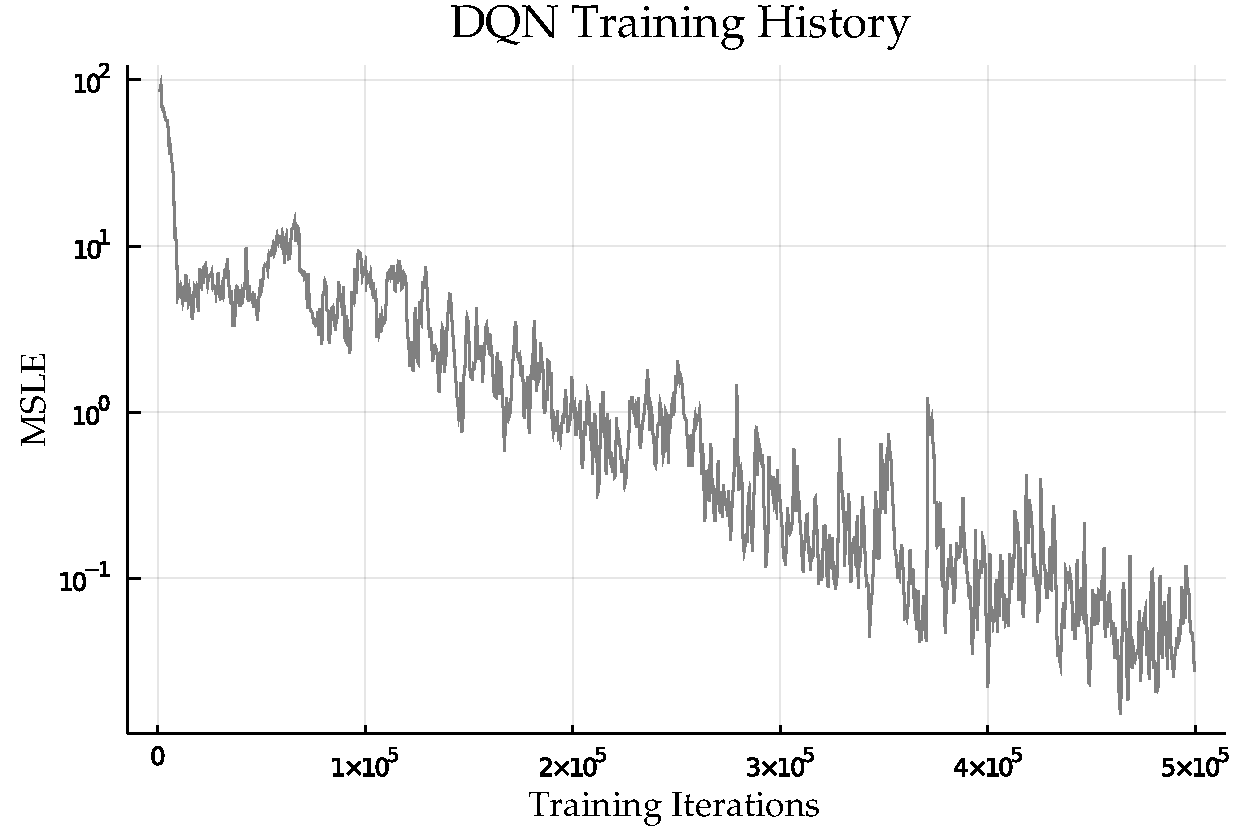
\includegraphics[width=\textwidth]{figures/distribution_over_failures/dqn_training_history.pdf}
        \caption{MSLE between neural network and ground truth during training.}
        \label{fig:gridworld_pfail_dqn_training_hist}
\end{figure}

\begin{figure*}
    \centering
    \begin{subfigure}[b]{0.49\textwidth}
        \centering
        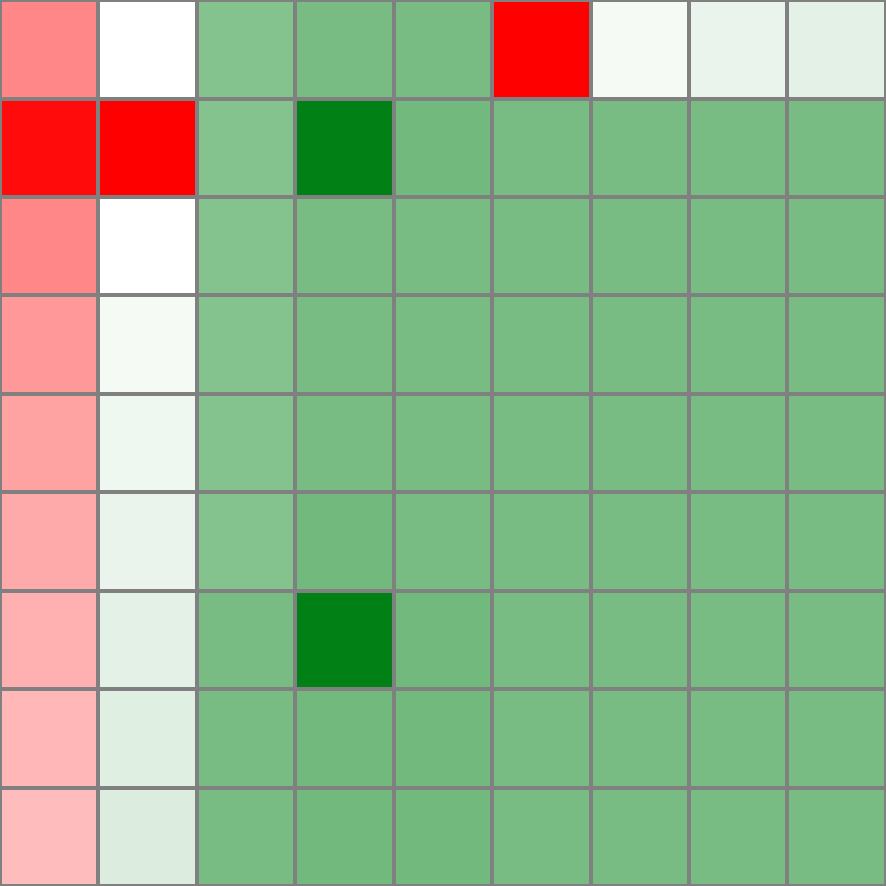
\includegraphics[width=0.78\textwidth]{figures/distribution_over_failures/vi_pfail.pdf}
        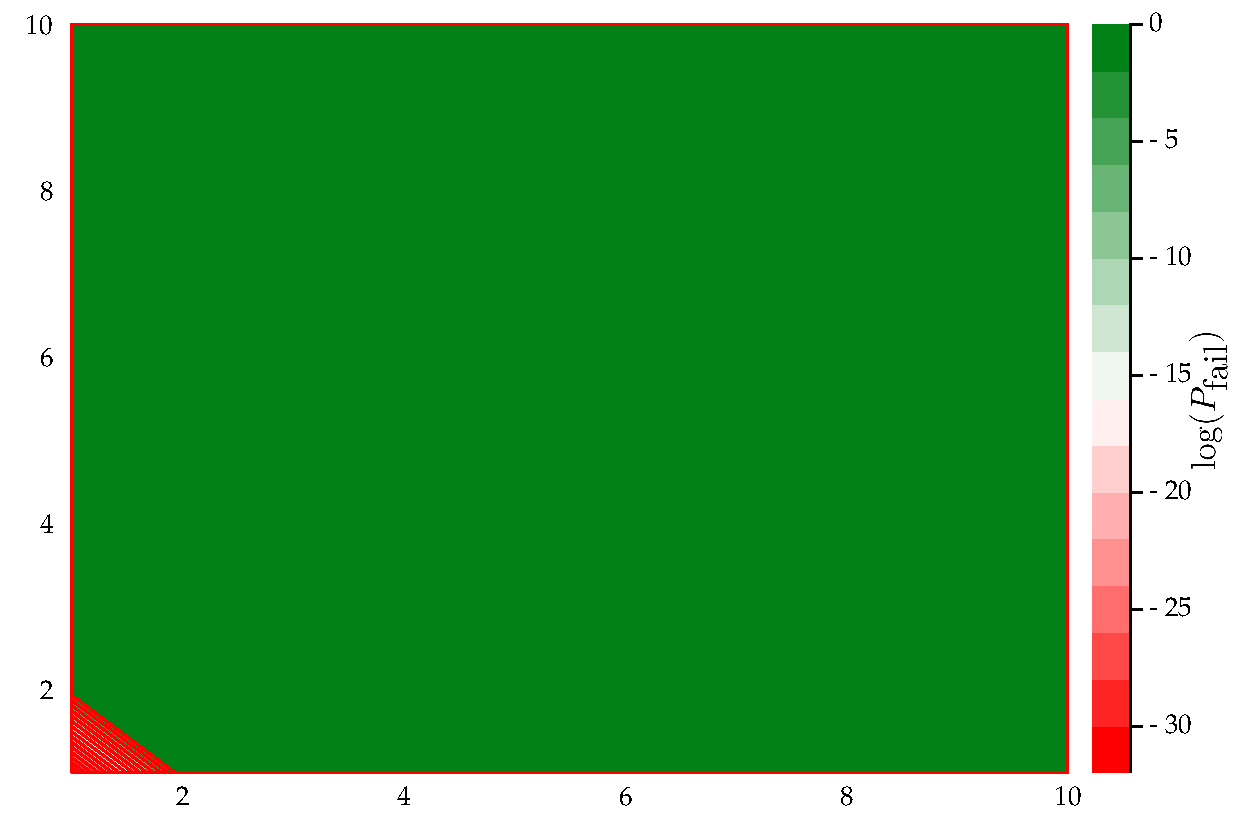
\includegraphics[width=0.17\textwidth, trim={18.4cm, 1cm, 0, 0}, clip]{figures/distribution_over_failures/colorbar.pdf}
        \caption{$P_{\rm fail}$ ground truth.}
        \label{fig:vi_pfail}
    \end{subfigure}
    \hfill
    \begin{subfigure}[b]{0.49\textwidth}
        \centering
        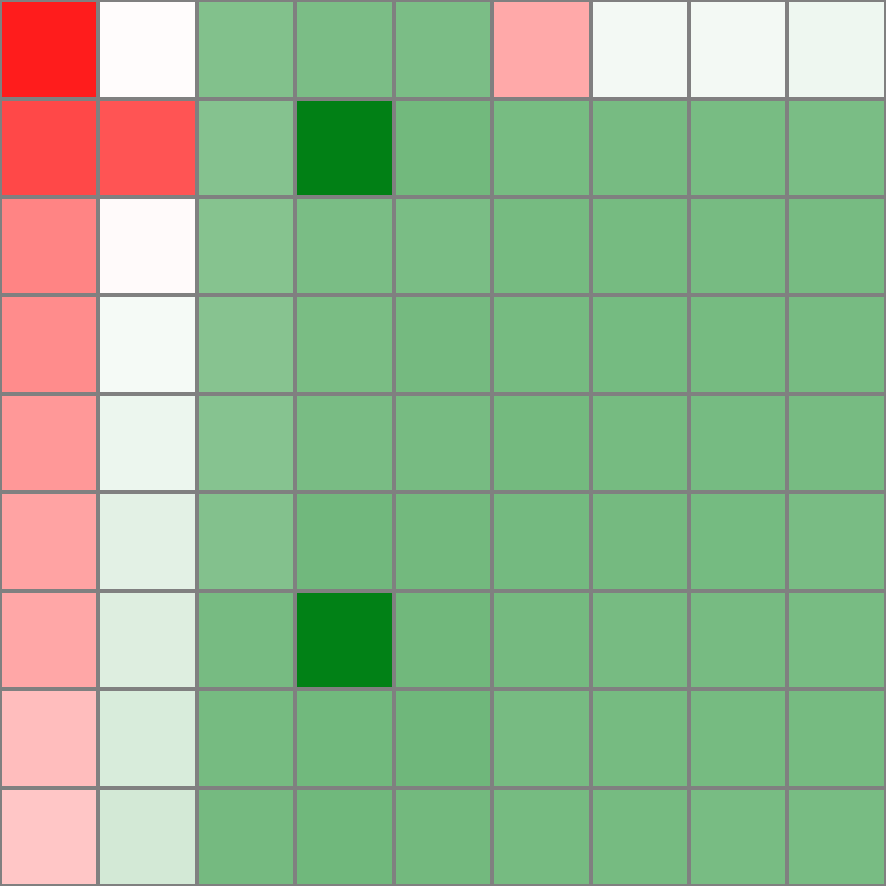
\includegraphics[width=0.78\textwidth]{figures/distribution_over_failures/dqn_pfail.pdf}
        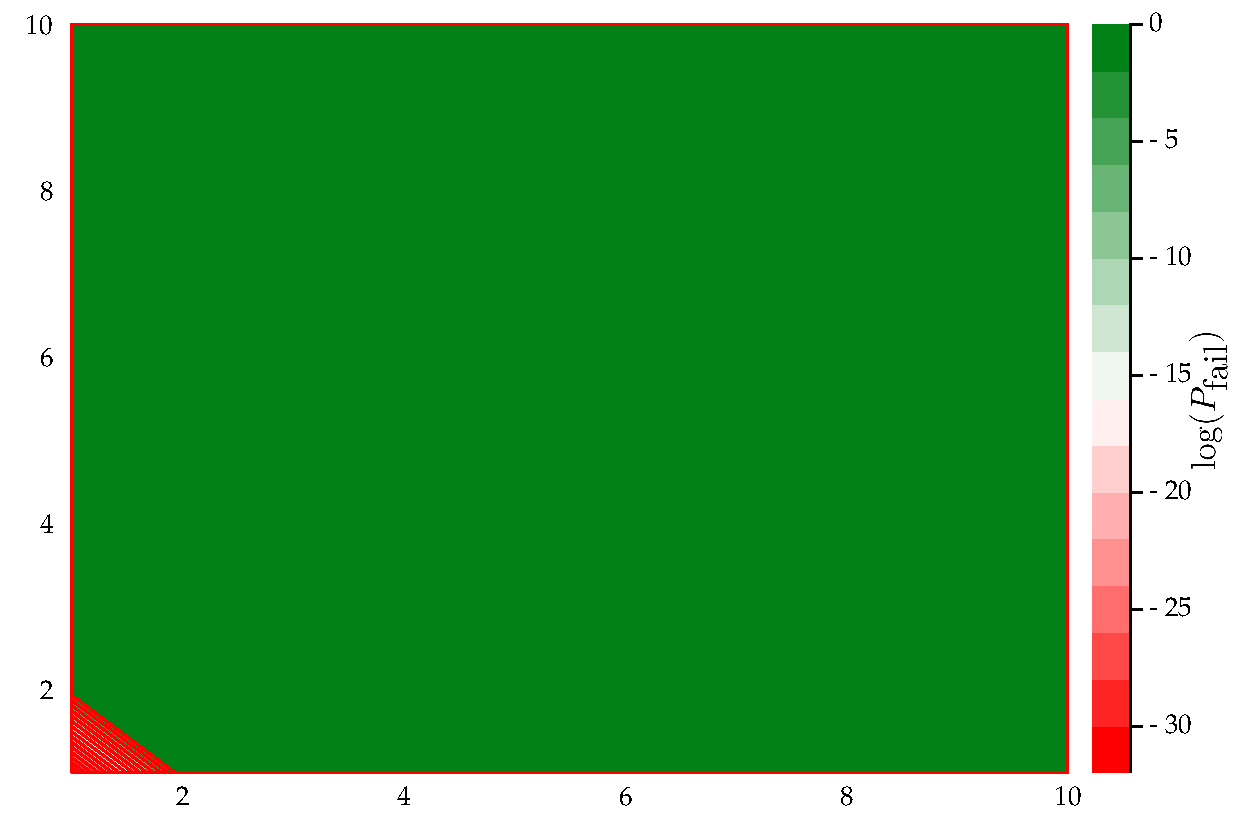
\includegraphics[width=0.17\textwidth, trim={18.4cm, 1cm, 0, 0}, clip]{figures/distribution_over_failures/colorbar.pdf}
        \caption{$P_{\rm fail}$ from DQN.}
        \label{fig:dqn_approx_pfail}
    \end{subfigure}
    \caption{Comparison of $P_{\rm fail}$ between DQN and exact value iteration.}
    \label{fig:dqn_comp_ground_truth}
\end{figure*}

We now compare the proposal distribution $q^*(x \mid s)$ (with $P_{\rm fail}(s)$ computed through exact value iteration and DQN) to the Monte Carlo and cross entropy method baselines. The failure rate and log-likelihood of failures is reported in \cref{tab:ch5_gridworld_results}. The cross entropy method is able to significantly increase the rate of discovered failures, but the average log-likelihood of those failures is much smaller than the most commonly observed failures. Using $q^*$ with both DQN estimation and exact value iteration maximizes the rate of failures discovered while retaining a relatively high likelihood of failure trajectories. 

\cref{fig:gridworld_pfail_vs_samples} shows how each technique performs when used to estimate the probability of failure. Monte Carlo sampling ultimately gives an accurate estimate but does not observe a failure for the first ~\num{2000} samples. The cross entropy method observes samples early on, but due to their low log-probability they are give small importance sampling weights and therefore create an erroneous estimate. The DQN and value iteration approaches both quickly converge to a good estimate of the probability of failure with value iteration performing slightly better. The reason the value iteration estimate has any variance at all is because the agent is initialized to a random place on the grid for each sample. 


\begin{table}
    \centering
    \caption{Simple gridworld failure results.}
    \label{tab:ch5_gridworld_results}
    \begin{tabular}{@{}lll@{}} 
        \toprule
        \textbf{Method} & \textbf{Failure Rate} & \textbf{Log Likelihood}\\
        \midrule
        Monte Carlo & \num{0.001} \pm \num{0.001} & \num{-8.013} \pm \num{0.0} \\
        Cross entropy method & \num{0.255} \pm \num{0.014} & \num{-36.431} \pm \num{2.05} \\
        DQN & \num{0.98} \pm \num{0.004} & \num{-10.654} \pm \num{0.51} \\
        Value iteration & \num{1.0} \pm \num{0.0} & \num{-11.375} \pm \num{0.604} \\
        \bottomrule
    \end{tabular}
\end{table}

\begin{figure}
        \centering
        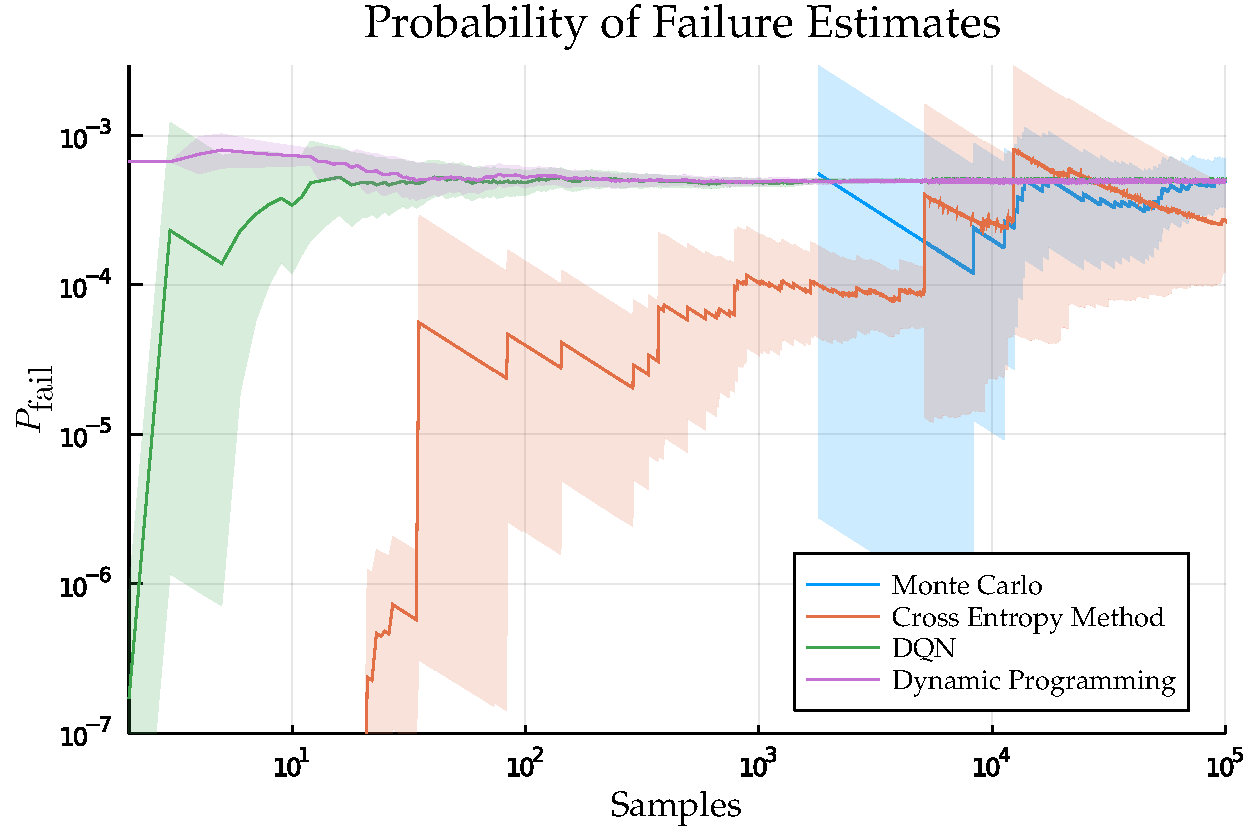
\includegraphics[width=\textwidth]{figures/distribution_over_failures/pfail_gridworld.pdf}
        \caption{Comparison of techniques for $P_{\rm fail}$ estimation for the simple gridworld.}
        \label{fig:gridworld_pfail_vs_samples}
\end{figure}



\subsection{T-intersection Scenario}
\label{sec:ch5_Tint}
We now turn to the more complex problem of discovering failures in the autonomous driving policy of the ego vehicle in the T-intersection scenario. The problem is more challenging due to the longer time horizon  and the continuous state space. In each episode, the agents are initialized with random positions in the range [\SI{5}{m}, \SI{35}{m}] (with respect to the start of their lane) and random velocities in the range [\SI{10}{m/s}, \SI{20}{m/s}]. The adversarial agent is initialized on the left with a random turn intention and match turn signal. Any initial condition that had a collision without any disturbance was not used in the analysis. 

In addition to all the baselines and DQN, we use local approximation value iteration to estimate the probability of failure. We discretize the state space into \num{30} position points and \num{10} velocity points for each vehicle, resulting in a total of \num{360000} states. To focus the sample points on the most interesting regions of the state space (i.e. the positions before and immediately after the intersection and the reachable range of velocities), we uniformly discretize the adversary position between [\SI{0}{m}, \SI{75}{m}] an the ego vehicle between [\SI{15}{m}, \SI{75}{m}], and the velocity between [\SI{0}{m/s}, \SI{20}{m/s}]. Interpolation was done using bilinear interpolation over the grid of states. 


The failure rates and average failure log-likelihood is shown in \cref{tab:ch5_2car_results}. The uniform sampling distribution is able to increase the failure rate but at the cost of low-likelihood failures. The cross entropy method does not perform much better than basic Monte Carlo sampling. Both techniques that use $q^*$ have significantly higher failure rates and relatively high log-likelihoods. When $P_{\rm fail}(s)$ is estimated using DQN, we get a higher failure rate and log-likelihood compared to local approximation value iteration. Likewise, in the estimate of the probability of failure (\cref{fig:ch5_2car_pfail_estimation}) the DQN approach seems to have less variance than local approximation value iteration. 

Local approximation value iteration may perform worse than DQN due to the requirement of such a coarse discretization of the state space. Small features in the landscape of $P_{\rm fail}(s)$ that are captured by a neural network may be missed using a coarse grid and linear interpolation, leading to less efficient proposal distribution.

\begin{table}
    \centering
    \caption{Two car T-intersection results.}
    \label{tab:ch5_2car_results}
    \begin{tabular}{@{}lll@{}} 
        \toprule
        \textbf{Method} & \textbf{Failure Rate} & \textbf{Log Likelihood}\\
        \midrule
        Monte Carlo & \num{0.0} \pm \num{0.0} & \num{-9.352} \pm \num{0.372} \\
        Uniform sampling & \num{0.087} \pm \num{0.009} & \num{-97.703} \pm \num{2.822} \\
        Cross entropy method & \num{0.007} \pm \num{0.003} & \num{-10.416} \pm \num{0.313} \\
        DQN & \num{0.365} \pm \num{0.015} & \num{-9.562} \pm \num{0.16} \\
        Local Approximation VI & \num{0.214} \pm \num{0.013} & \num{-11.45} \pm \num{0.4} \\
        \bottomrule
    \end{tabular}
\end{table}

\begin{figure}
        \centering
        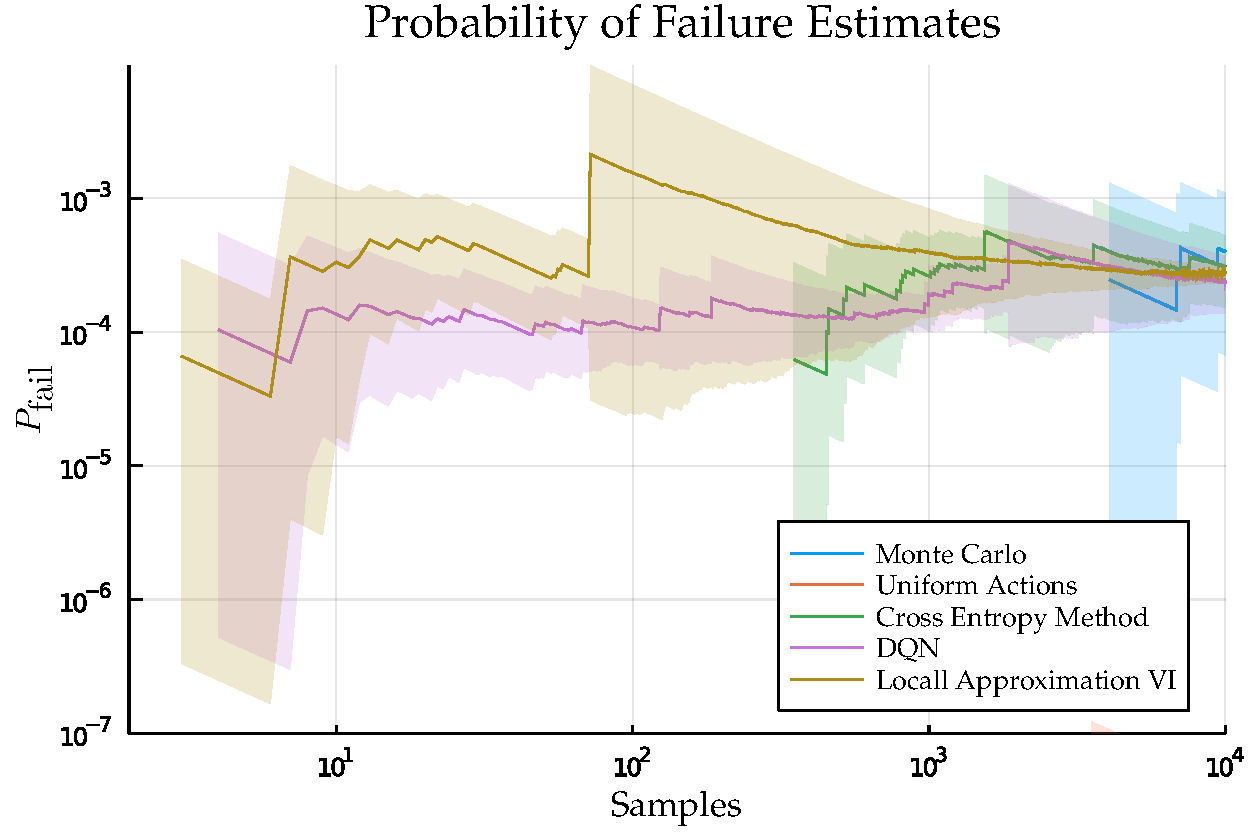
\includegraphics[width=\textwidth]{figures/distribution_over_failures/pfail_2car_left.pdf}
        \caption{Comparison of techniques for $P_{\rm fail}$ estimation for the 2-car T-intersection scenario.}
        \label{fig:ch5_2car_pfail_estimation}
\end{figure}

\section{Discussion}

% Summary of what the chapter was about
In this chapter we argue that safety validation algorithms that optimize to find individual failure trajectories are insufficient for obtaining a diverse set of likely failures and for estimating the failure probability. One solution is to approximate the distribution over failures and use it as a stochastic policy for choosing disturbances. We showed that a distribution that is proportional to the probability of failure can be an efficient proposal distribution, and is optimal when applied to a deterministic environment. This insight reduces the problem of approximating the distribution over failure to estimating the probability of failure for each state and disturbance pair. 

When we invoke the Markov assumption, we show that the probability of failure is the solution to a Bellman equation which can be solved exactly or approximately depending on the size of the state and disturbance space. We showed that a modified version of DQN can also approximate the probability of failure even when those probabilities are extremely small. Through experiments with the gridworld and T-intersection scenarios, we demonstrate that our proposal distribution is able to find more failures, find failures with high log-likelihood, and better estimate the probability of failure than baseline techniques. 

% Relation to other work 
The work presented in this chapter is related to several other approaches. Adaptive stress testing (AST)~\cite{lee2015adaptive,koren2018adaptive,corso2019adaptive,koren2019efficient} also frames the safety validation problem as a Markov decision process and uses reinforcement learning to find likely failures. AST optimizes for the most-likely failure and has been shown converge to individual failure modes~\cite{corso2019adaptive}. The field of statistical model checking~\cite{agha2018survey} deals with estimating the probability of failure of a system but relies on basic sampling techniques with an emphasis on hypothesis testing for making probabilistic safety claims.

There is a large amount of literature where importance sampling has been applied to estimate the probability of failure (some of it is covered in \cref{sec:is}). Most relevant to this chapter is the work by \textcite{Chryssanthacopoulos2010}, where they apply a similar state-based importance sampling distribution to estimate the probability of failure of an aircraft collision avoidance system. The probability of failure is roughly estimated using local approximation value iteration and used to construct an importance sampling distribution. They do not, however, analyze the variance of the estimator or propose scalable techniques for estimating the probability of failure.  \textcite{uesato2019rigorous} also use an estimate of the probability of failure to choose initial conditions that cause an agent to failure. They do not extend their work to sequential decision making, but it is interesting to note that they derived the optimal sampling distribution for a single step stochastic simulator to be proportional to the $\sqrt{P_{\rm fail}}$. This insight does not, however, appear to be directly applicable to deriving the optimal state-dependent sampling distribution for sequential problems.

% Limitations and introduction to the next chapter
One of the biggest challenges to applying this technique to large problems is the scalability to larger state and disturbance spaces. Value iteration approaches explicitly iterate over states, while the quality of a neural network estimate will depend on having experience samples that sufficiently cover the state space. In the next chapter we introduce a scene decomposition technique that can improve the scalability of this technique. 